 \iffalse
\chapter{2014}
\author{EE24BTECH11021 - Eshan Ray}
\section{me}
\fi
    \item Choose the most appropriate phase from the options given below to complete the following sentence.\\ \\
    The aircraft \dots take off as soon as its flight plan was filed.    
    \begin{enumerate}
        \item is allowed to
        \item will be allowed to
        \item was allowed to
        \item has been allowed to
    \end{enumerate}
    \item Read the statements $\colon$ \\ \\
    All women are entrepreneurs.\\
    Some women are doctors. \\ \\
    Which of the following conclusions can be logically inferred from the above statements?
    \begin{enumerate}
        \item All women are doctors
        \item All doctors are entrepreneurs
        \item All entrepreneurs are women
        \item Some entrepreneurs are doctors
    \end{enumerate}
    \item Choose the most appropriate word from the options given below to complete the following sentence.\\ \\
    Many ancient culture attributed disease to supernatural causes. However, modern science has largely helped \dots such notions.
    \begin{enumerate}
        \item impel
        \item dispel
        \item propel
        \item repel
    \end{enumerate}
    \item The statistics of runs scored in a series by four batsman are provided in the following table. Who is the most \underline{consistent} batsman of these four?
	
    \begin{table}[H]    
  \centering
  \begin{tabular}[12pt]{ |c| c| c|}
    \hline
	\textbf{Batsman}  & \textbf{Average} & \textbf{Standard Deviation} \\
    \hline
	$K$ &  $31.2$ & $5.21$  \\
    \hline 
	$L$ &  $46.0$ & $6.35$\\
    \hline
	$M$ &  $54.4$ & $6.22$ \\  
    \hline
    	$N$ &  $17.9$ & $5.90$ \\
    \hline         
\end{tabular}

  \label{tab1.1.9.2}
\end{table}
    \begin{enumerate}
        \item $K$
        \item $L$
        \item $M$
        \item $N$
    \end{enumerate}
    \item What is the next number in the series?\\ \\
        $12\quad 35\quad81\quad173\quad357\quad\dots$
    \item Find the odd one from the following group $\colon$ \\ \\
        $W,E,K,O\quad I,Q,W,A\quad F,N,T,X\quad N,V,B,D$
     \begin{enumerate}
        \item $W,E,K,O$
        \item $I,Q,W,A$
        \item $F,N,T,X$
        \item $N,V,B,D$
    \end{enumerate}
    \item For submitting tax returns, all resident males with annual income below $Rs\,10\,lakh$ should fill up Form $P$ and all resident females with income below $Rs\,8\,lakh$ should fill Form $Q$. All people with incomes above $Rs\,10\,lakh$ should fill up Form $R$, except non-residents with income above $Rs\,15\,lakhs$, who should fill up Form $S$. All others should fill Form $T$. An example of a person who should fill Form $T$ is 
        \begin{enumerate}
            \item a resident male with annual income of $Rs\,9\,lakh$
            \item a resident female with annual income of $Rs\,9\,lakh$
            \item a non-resident male with annual income of $Rs\,16\,lakh$
            \item a non-resident female with annual income of $Rs\,16\,lakh$
        \end{enumerate}
    \item A train that is $280$ metres long, travelling at a uniform speed, crosses a platform in $60$ seconds and passes a man standing on the platform in $20$ seconds. What is the length of the platform in metres?
    \item The exports and imports \brak{in\,crores\,of\,Rs.} of a country from $2000$ to $2007$ are given in the following bar chart. If the trade deficit is defined as excess of imports over exports, in which year is the trade deficit $\frac{1}{5}th$ of the exports? 
\begin{figure}[H]
    \centering
	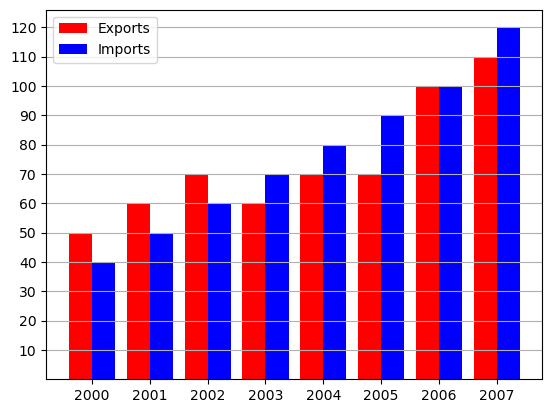
\includegraphics[width=0.5\textwidth]{GATE-yearwise/EE24BTECH11021/plots/plot.png}
    \label{fig:plot}
    \end{figure}
    \begin{enumerate}
        \item $2005$
        \item $2004$
        \item $2007$
        \item $2006$
    \end{enumerate}
    
    
    \item You are given three coins $\colon$ one has heads on both faces, the second has tails on both faces, and the third has a head on one face and a tail on the other. You choose a coin at random and toss it, and it comes up heads. The probability that the other face tails is
    \begin{enumerate}
        \item $\frac{1}{4}$
        \item $\frac{1}{3}$
        \item $\frac{1}{2}$
        \item $\frac{2}{3}$
    \end{enumerate}
    \item Given that the determinant of the matrix $\myvec{1&3&0\\2&6&4\\-1&0&2}$ is $-12$, the determinant of the matrix $\myvec{2&6&0\\4&12&8\\-2&0&4}$ is
    \begin{enumerate}
        \item $-96$
        \item $-24$
        \item $24$
        \item $96$
    \end{enumerate}
    \item $\lim_{x\to0}\frac{x-\sin x}{1-\cos{x}}$ is
        \begin{enumerate}
            \item $0$
            \item $1$
            \item $3$
            \item not defined
        \end{enumerate}
    \item The argument of the complex number $\frac{1+i}{1-i}$, where $i=\sqrt{-1}$, is
            \begin{enumerate}
                \item $-\pi$
                \item $-\frac{\pi}{2}$
                \item $\frac{\pi}{2}$
                \item $\pi$
            \end{enumerate}
